\documentclass[conference]{IEEEtran}

\usepackage{cite}
\usepackage{amsmath}
\usepackage{amssymb}
\usepackage{graphicx}
\usepackage{booktabs}
\usepackage{multirow}
\usepackage{array}
\usepackage{url}
\usepackage{listings}
\usepackage[hidelinks]{hyperref}

\lstset{
basicstyle=\ttfamily\scriptsize,
columns=fullflexible,
keepspaces=true,
showstringspaces=false,
frame=single
}

\title{RTDL: A Python-Hosted Ray-Tracing DSL for Non-Graphical Spatial Workloads}

\author{
\IEEEauthorblockN{Rubao Lee}
\IEEEauthorblockA{\texttt{lee.rubao@ieee.org}}
}

\begin{document}
\maketitle

\begin{abstract}
Ray tracing (RT) is widely used for image synthesis because it solves
hierarchical geometric search efficiently. The same capability is attractive
for non-graphical workloads such as spatial joins, point-in-polygon tests, and
geometric candidate generation, but direct use of RT runtimes still requires
backend-specific engineering. We present RTDL (Ray-Tracing Domain Language), a
Python-hosted DSL and compiler/runtime system for expressing such workloads
once and lowering them to multiple backends while preserving explicit
semantics. RTDL separates authored kernel meaning from backend-specific
execution details such as acceleration-structure construction, launch state,
buffer layout, and result materialization. We evaluate RTDL on the RayJoin
workload family using stable real-data packages and controlled scalability
studies. Across the accepted package surfaces, RTDL preserves exact row-level
parity among a native C++ oracle, Embree, OptiX, and an external PostGIS
reference. On the main long County--Zipcode point-in-polygon workload reported
in this paper, RTDL with Embree and RTDL with OptiX both outperform PostGIS on
the published prepared-execution and repeated-call boundaries. The result is a
reproducible, multi-backend evaluation showing that a programmable RT
language/runtime stack can be a credible way to build non-graphical
ray-tracing workloads.
\end{abstract}

\begin{IEEEkeywords}
domain-specific language, ray tracing, spatial joins, Embree, OptiX, PostGIS,
RayJoin, reproducibility
\end{IEEEkeywords}

\section{Introduction}

The recent proliferation of hardware-accelerated ray-tracing (RT) cores and
high-performance traversal kernels has transformed graphics, but their
potential for non-graphical spatial computing remains underexploited.
Operations such as spatial joins, point-in-polygon tests, and geometric
candidate filtering are natural fits for BVH-style traversal and intersection
machinery. In practice, however, exploiting that hardware still requires
backend-specific engineering around memory layout, launch configuration,
payload conventions, and numerical boundary semantics. The programming burden
is especially high when the goal is to preserve the same workload semantics
across CPU and GPU execution paths.

RTDL is intended to reduce that programming burden by raising the authoring
surface from backend-specific APIs to a compact kernel DSL while retaining
multiple execution backends. The language is hosted in Python, but its purpose
is not scripting convenience alone. Its purpose is to let an author specify
geometric inputs, traversal intent, refine predicates, and output rows once,
then lower that kernel into controlled runtime paths with comparable semantics.
The central question of this paper is whether such an abstraction can remain
useful and defensible when evaluated on a demanding, already-published workload
family.

RayJoin is the right target for that evaluation because it exercises exactly
the class of workloads RTDL is meant to support: non-graphical ray-tracing
queries over spatial data with both correctness and performance demands. This
paper therefore does two things. First, it presents RTDL as a language/runtime
design for this workload class. Second, it evaluates RTDL on a carefully scoped
RayJoin-oriented package consisting of stable real-data cases and controlled
scaling studies. The scope is intentionally narrower than a full paper-identical
reproduction: unavailable dataset families remain deferred, and the current
overlay result remains a seed-generation surface rather than full polygon
materialization.

This paper makes the following contributions:
\begin{enumerate}
\item \textbf{The RTDL System}: We introduce a Python-hosted DSL and compiler
that lowers high-level spatial kernels into a backend-independent intermediate
representation, separating kernel semantics from backend-specific traversal and
scheduling.
\item \textbf{Multi-Backend Runtime}: We describe an extensible runtime
architecture that supports execution across Intel Embree (CPU), NVIDIA OptiX
(GPU), and a native C++ semantic oracle.
\item \textbf{Cross-System Correctness Methodology}: We establish a rigorous
validation framework that ensures exact, row-level parity across heterogeneous
execution paths, utilizing PostGIS as an external industrial baseline for
real-data packages.
\item \textbf{RayJoin-Oriented Evaluation}: We provide a reproducible,
multi-backend evaluation of RayJoin-style LSI, PIP, and overlay-seed workloads
on stable datasets, demonstrating that RTDL can preserve exact semantics while
targeting heterogeneous RT backends.
\end{enumerate}

\section{Related Work}

\subsection{Spatial Join Systems}

RayJoin is the closest direct comparison point for this paper because RTDL is
explicitly evaluated against its workload family, artifact structure, and
reporting surfaces~\cite{rayjoin}. PostGIS remains the most important external
reference in the current RTDL evaluation because it provides a widely used
industrial spatial database with indexed spatial predicates and well-understood
geometry semantics~\cite{postgis}. GeoSpark SQL represents a different design
point: it exposes SQL-level spatial operations on top of a distributed
Spark/Hive execution substrate rather than a backend-portable kernel
language~\cite{geosparksql}. Other widely used distributed spatial systems, such
as SpatialHadoop and Apache Sedona, occupy the same broad system class even
though they expose different storage and execution tradeoffs~\cite{spatialhadoop,sedona}.
RTDL differs from all of these classes of systems. It is
not a database, and it is not a paper-specific one-off implementation. Instead,
it aims to express non-graphical ray-tracing workloads through a constrained
kernel language and then lower them into multiple execution backends while
keeping explicit correctness contracts.

\subsection{Compiler and DSL Context}

RTDL also relates to compiler-backed domain-specific systems such as
Halide~\cite{halide} and TVM~\cite{tvm}. Those systems separate high-level
computation intent from lower-level schedule or backend realization and are
therefore important precedents for RTDL's own authored-kernel to backend-plan
split. The difference is domain focus. Halide and TVM center image-processing
and tensor-operator pipelines, whereas RTDL centers geometric candidate
generation, refine predicates, and emitted join rows. The relevant design
pressure is therefore not only optimization, but exact spatial semantics across
heterogeneous backends.

\subsection{Ray-Tracing Runtime Context}

At the runtime layer, RTDL builds on ray-tracing infrastructure rather than
reimplementing traversal from scratch. Embree provides the validated CPU
ray-tracing kernel framework~\cite{embree}, while OptiX provides the reported
GPU execution path in this paper~\cite{optix}. RTDL's contribution is not a new
traversal engine. The contribution is the language/runtime boundary, the native
oracle, and the reproducible multi-system evaluation built on top of these
runtimes.

\section{What Ray Tracing Is and Why It Matters Beyond Graphics}

In graphics, ray tracing answers visibility questions by traversing geometric
hierarchies quickly. Rays, bounding-volume hierarchies, and fast intersection
kernels make it practical to search complex geometric scenes without checking
every primitive pair directly. The same basic pattern also appears in
non-graphical workloads. A spatial join, for example, can often be expressed as
a broad-phase search for candidate geometry pairs followed by an exact refine
step on the surviving candidates.

This observation is what makes ray tracing interesting for spatial computing.
Workloads such as line-segment intersection, point-in-polygon, overlap
candidate generation, and geometric counting all involve the same kind of
hierarchical search that RT systems already accelerate well. Systems such as
RayJoin~\cite{rayjoin} demonstrate that this mapping is not merely conceptual:
ray-tracing cores can be used effectively for spatial join work.

The problem is that using RT backends directly still exposes a great deal of
backend-specific engineering. Developers must reason about acceleration
structures, payload/state conventions, memory layout, launch details, and
boundary behavior separately for CPU and GPU paths. RTDL addresses that problem
instead of trying to replace the underlying traversal engines.

\subsection{RayJoin as the First Application Target}

RayJoin is the right first target for RTDL because it exercises the exact class
of workloads RTDL is meant to support~\cite{rayjoin}.

The current RTDL paper does not claim a paper-identical reproduction of every
RayJoin dataset family. Instead, it uses RayJoin as the workload and evaluation
reference point for a more language/runtime-oriented question: can one authored
kernel surface survive lowering to multiple RT backends while preserving exact
semantics and producing honest performance claims?

The evaluation surface mirrored from RayJoin includes three workload families:
\begin{itemize}
\item \textbf{LSI}: line-segment intersection style joins,
\item \textbf{PIP}: point-in-polygon style joins,
\item \textbf{Overlay}: currently represented in RTDL as an
\textit{overlay-seed evaluation}, which identifies intersecting polygon pairs
without full geometry materialization.
\end{itemize}

For this work, RayJoin Figure~13 and Figure~14 are represented through
controlled synthetic studies, while RayJoin Table~3, Table~4, and Figure~15
are represented through validated results on stable dataset packages.

\section{Why RTDL and How It Works}

\subsection{Why a DSL Is Needed}

The central design claim of RTDL is that non-graphical RT workloads should be
programmable at the workload level rather than at the backend-API level.
Without such an abstraction, every new workload must be translated manually
into backend-specific setup code, traversal configuration, payload plumbing,
buffer layout, and result marshaling. That makes correctness difficult to
compare across systems and slows down experimentation.

RTDL therefore tries to keep the authored surface close to the workload itself:

\begin{itemize}
\item which geometries are inputs,
\item which side is probe or build,
\item what traversal is intended,
\item what refine predicate defines final truth,
\item which fields belong in the emitted rows.
\end{itemize}

The backend-specific execution details are still present, but they move below
the language boundary instead of staying in every authored workload.

\subsection{Language Surface}

RTDL is authored from Python through a constrained kernel DSL. A user writes a
kernel by declaring typed inputs, traversal intent, refine predicates, and
output fields. The intent is that authors specify workload meaning rather than
backend launch details. The same language surface currently supports six
implemented workloads in the repository, but the RayJoin-facing slice of this
paper focuses on LSI, PIP, and overlay.

\subsection{Representative Kernel}

Listing~\ref{lst:pip} shows the shape of an RTDL PIP kernel. The author
declares probe/build inputs, asks for BVH traversal, selects a refine
predicate, and specifies the emitted row schema. Backend-specific details such
as Embree scene construction, OptiX launch state, and row marshaling remain
outside the authored kernel.

\begin{lstlisting}[caption={Representative RTDL PIP kernel.},label={lst:pip}]
@rt.kernel(backend="rtdl", precision="float_approx")
def point_in_counties():
    points = rt.input("points", rt.Points, role="probe")
    polygons = rt.input("polygons", rt.Polygons, role="build")
    candidates = rt.traverse(points, polygons, accel="bvh")
    hits = rt.refine(
        candidates,
        predicate=rt.point_in_polygon(exact=False,
                                      boundary_mode="inclusive"),
    )
    return rt.emit(hits, fields=["point_id", "polygon_id", "contains"])
\end{lstlisting}

\subsection{Compiled Representation and Lowering}

RTDL lowers authored kernels into a compiled-kernel representation that
separates language semantics from backend realization. The lowering path remains
RayJoin-oriented in the current codebase: it maps geometry roles, candidate
generation, refine predicates, and emitted rows into backend-specific execution
plans. In practice, the lowered form records the probe/build role assignment,
the traversal primitive to invoke, the refine predicate family, precision and
boundary-mode settings, and the emitted row schema. The backend adapters then
translate that representation into concrete execution state such as Embree
scenes, OptiX launch parameters, native buffers, and row marshaling logic. This
allows the same kernel to execute against a semantic oracle, a CPU Embree
runtime, and a GPU OptiX runtime without changing the authored kernel surface.

\subsection{Execution Backends}

The evaluated backends for this paper are:
\begin{itemize}
\item \textbf{Native C/C++ oracle}: the semantic ground truth for the reported
results.
\item \textbf{Embree}: the primary validated CPU backend.
\item \textbf{OptiX}: the validated GPU backend on the Linux workstation in
Table~\ref{tab:environment}.
\end{itemize}

The Vulkan backend remains in the repository, but the paper's main performance
story focuses on Embree and OptiX because those are the mature high-performance
backends on the accepted long exact-source surface.

\subsection{Execution Pipeline}

The execution path is conceptually simple even though the backend
implementations are not. RTDL first compiles the authored kernel into a
backend-independent representation that records geometry roles, traversal
structure, refine predicate, and emitted fields. The runtime then normalizes
input geometry, invokes the selected backend, and converts the returned native
rows into the requested user-facing representation. The crucial discipline in
this paper is that all reported real-data results are checked against the
native oracle and, for the validated real-data packages, against PostGIS as an
external reference.

This separation between authored kernel, lowered representation, and runtime
adapter is the main systems contribution of RTDL. It keeps semantic decisions
visible at the language level while still allowing backend-specific execution
strategies underneath. The resulting paper is therefore not just a benchmark of
Embree or OptiX; it is an evaluation of whether one authored workload surface
can survive translation into multiple RT backends without drifting
semantically.

\begin{figure}[t]
\centering
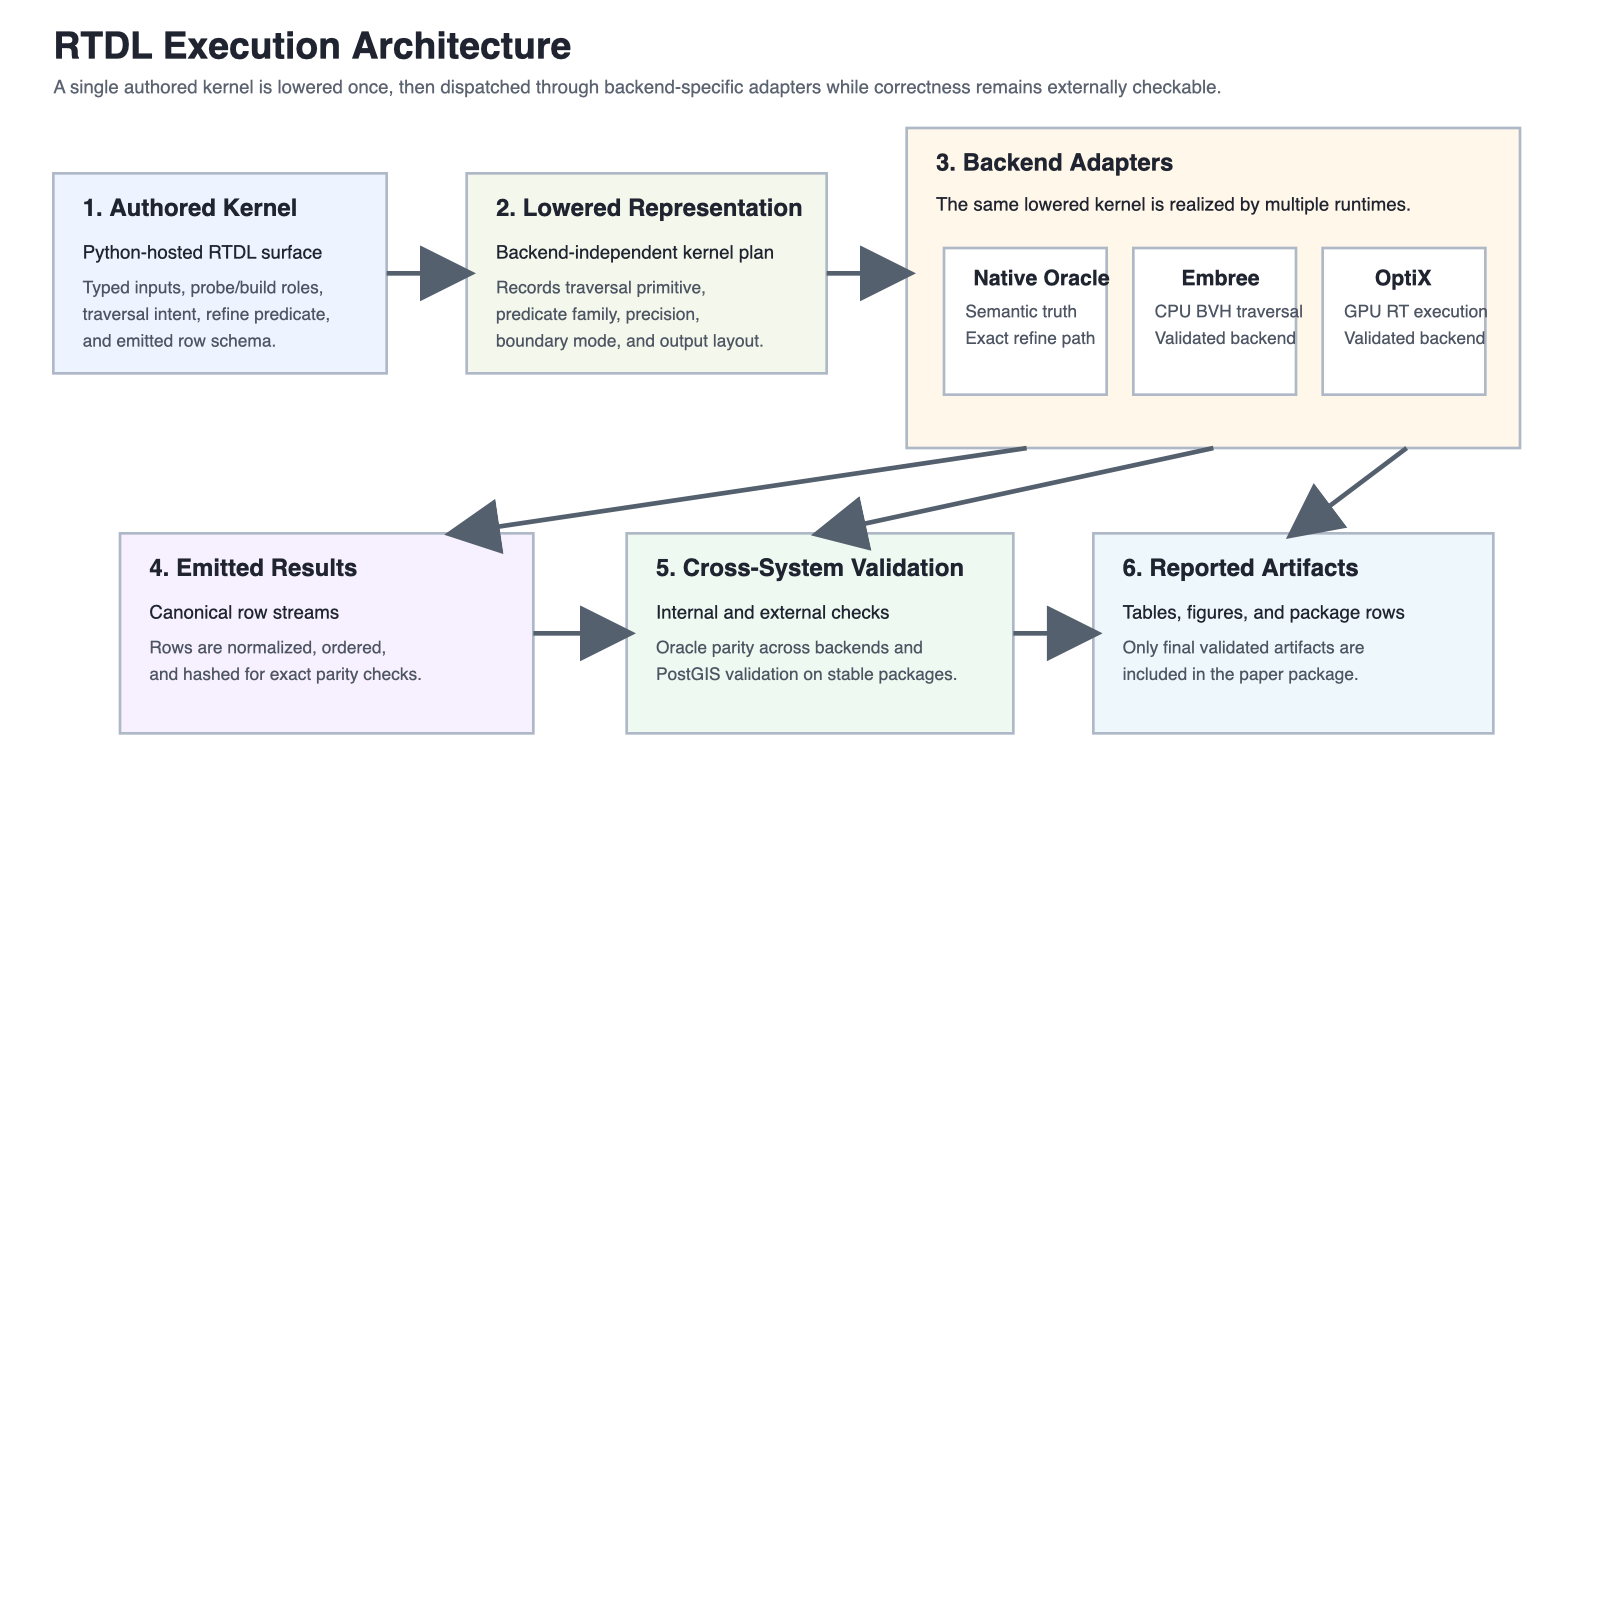
\includegraphics[width=\columnwidth]{rtdl_paper_assets/figures/rtdl_architecture.png}
\caption{RTDL execution architecture. A single authored kernel is lowered into a backend-independent representation, dispatched through backend adapters, and checked through emitted-row parity and external validation.}
\label{fig:rtdl-architecture}
\end{figure}

\section{Design Considerations and Evaluation Methodology}

\subsection{Design Considerations}

Three design considerations drive the current RTDL package.

First, semantic consistency is more important than backend-local cleverness.
The paper compares systems that execute related geometric work under different
runtime conditions, so the language/runtime layer must make boundary modes,
refine predicates, and emitted rows explicit enough to compare honestly.

Second, RTDL must separate broad-phase candidate generation from final truth.
That principle shaped the mature positive-hit point-in-polygon paths reported
here. Embree and OptiX both use backend-specific candidate generation, but the
reported accepted paths keep final inclusive truth on the host through exact
finalization.

Third, the Python host is allowed to orchestrate but should not repeatedly do
bulk geometry work on the hot path. The strongest current performance wins only
appeared after the runtime began reusing prepared executions and prepacked
geometry instead of rebuilding them unnecessarily.

\subsection{Optimization Strategy}

The optimization story in this paper is therefore not ``replace PostGIS with a
single GPU kernel.'' It is a layered systems story.

At the backend level, RTDL relies on mature traversal runtimes such as Embree
and OptiX. At the language/runtime level, the main optimizations are:

\begin{itemize}
\item over-approximating backend candidate generation with host exact finalize,
\item prepared-execution reuse,
\item canonical-record and cached-prepared fast paths,
\item reuse of prepacked point and polygon buffers,
\item moving one-time launch costs out of repeated timed prepared execution
surfaces when that boundary already charges them to preparation.
\end{itemize}

These optimizations matter because the practical performance gap in a DSL
system often comes not from raw traversal speed, but from repeated packing,
binding, and result-materialization overhead around the backend itself.

\subsection{Correctness Method}

The correctness methodology is intentionally layered. The native C/C++ oracle
serves as the internal semantic ground truth. Embree and OptiX are checked
against that oracle. For validated real-data packages, PostGIS serves as an
external industrial reference. PostGIS queries are executed with indexed
GiST-assisted plans rather than brute-force SQL. For PIP, PostGIS positive-hit
queries are expanded into the same full-matrix RTDL truth semantics before
parity comparison.

The PIP parity path used in this paper is also more specific than a generic manual
point-in-polygon implementation. During development, a systematic external
comparison against PostGIS exposed remaining boundary/topology mismatches, so
the RTDL refine path adopted
GEOS-backed prepared-polygon \texttt{covers(point)} semantics for the native
oracle and Embree, and the reported OptiX overlay result was observed on a
GEOS-enabled build on the validated Linux host~\cite{geos}. This detail matters
because the paper claims exact parity with PostGIS on the validated packages,
not merely approximate geometric agreement. This does align RTDL's final refine
step more closely with the geometric engine family used by PostGIS, but that
alignment is intentional: the goal is to remove semantic ambiguity in the final
truth predicate, not to erase backend differences in candidate generation.

Parity is checked at the emitted-row level. In the validated artifacts, each
system produces a canonical row order, and the final row stream is hashed with
SHA-256. This paper therefore includes only cases whose final reported
artifacts established exact hash-level agreement across the compared systems.

\subsection{Experimental Scope}

This paper uses only final validated artifacts from the repository history. A
case is included only if it is already validated and clearly scoped. The paper
therefore distinguishes:
\begin{itemize}
\item \textbf{validated package}: a stable real-data package or synthetic
evaluation surface with completed parity and timing evidence,
\item \textbf{deferred-unavailable}: excluded because the public acquisition
path is unstable or unavailable,
\item \textbf{not claimed}: paper-identical or nationwide statements that the
current evidence does not justify.
\end{itemize}

All reported timings and parity statements in this paper come from the final
validated artifacts in the repository history. Earlier provisional or
superseded measurements are intentionally excluded.

\subsection{Experimental Environment}

Table~\ref{tab:environment} summarizes the host environment for the reported
four-system results. All four-system runs reported in this paper were executed
on the same Linux validation workstation.

\begin{table}[t]
\caption{Execution environment for the reported four-system package.}
\label{tab:environment}
\centering
\begin{tabular}{p{0.25\columnwidth}p{0.61\columnwidth}}
\toprule
Item & Value \\
\midrule
Host class & Linux validation workstation \\
OS & Ubuntu 24.04.4 LTS \\
CPU & Intel Core i7-7700HQ \\
Memory & 16\,GiB installed (about 15\,GiB usable) \\
GPU & NVIDIA GeForce GTX 1070 \\
Driver & 580.126.09 \\
CPU RT backend & Embree 4.3.0 \\
GPU RT backend & OptiX 9.0.0 \\
External checker & local PostgreSQL/PostGIS on the same host \\
GEOS role & exact prepared-polygon \texttt{covers(point)} path for validated PIP parity \\
\bottomrule
\end{tabular}
\end{table}

\subsection{Packages Used In This Paper}

The current manuscript is grounded in one bounded package family and one
stronger flagship evaluation surface. The bounded package includes County
$\bowtie$ Zipcode on \texttt{top4\_tx\_ca\_ny\_pa}, BlockGroup $\bowtie$
WaterBodies on \texttt{county2300\_s10}, and a bounded Australia
LKAU $\bowtie$ PKAU package. The strongest current flagship surface is the long
County $\bowtie$ Zipcode positive-hit PIP evaluation used throughout the later
RTDL backend-closure work. These packages were all validated on the Linux
validation workstation, and the bounded Australia package was staged from live
OSM Overpass way geometry and then frozen as the validated Australia
slice~\cite{overpass}.

\subsection{Overlay-Seed Contract}

RTDL's current overlay result is not full polygon materialization. The reported
surface is an \emph{overlay-seed evaluation} that records candidate pair
information and whether later LSI or PIP refine is required. This is the
current semantics-preserving surface compared against PostGIS in the validated
overlay package, and it is intentionally narrower than the full overlay output
reported in the original RayJoin paper.

\section{Current Evaluation Status}

The purpose of the current paper draft is to establish that RTDL is real,
programmable, and already strong enough to support meaningful non-graphical
ray-tracing workloads across multiple backends. The detailed experimental
artifact trail remains in the repository reports rather than in the paper body.
The current accepted result can therefore be stated compactly. RTDL preserves
exact emitted-row parity across the validated packages and uses PostGIS as the
external indexed reference on the main real-data surfaces. On the strongest
current long County $\bowtie$ Zipcode positive-hit PIP surface, Embree and
OptiX both beat PostGIS on the accepted prepared and repeated-call boundaries.
Vulkan is hardware-validated and parity-clean on that same surface, but slower.
That is enough for the paper's present purpose: to show that a Python-hosted
ray-tracing DSL/runtime stack is feasible, correct on the accepted package
surfaces, and already capable of competitive backend execution on the flagship
workload family.

\section{Relationship to RayJoin}

RayJoin provides the primary workload and evaluation reference for this paper.
RTDL does not attempt to replace RayJoin's contribution; instead, it asks a
different question: can the same workload family be expressed through a
programmable DSL/runtime surface while preserving exact semantics across
multiple execution backends? The answer reported here is deliberately scoped.
We mirror RayJoin's major workload categories and evaluation surfaces, but we
restrict the paper to stable, reproducible packages whose results can be
checked both against an internal oracle and, where appropriate, against
PostGIS. Unavailable or unstable dataset families are deferred rather than used
to support stronger reproduction claims than the evidence allows.

\subsection{Workload Surface}

The RTDL evaluation in this paper covers the same workload family categories
that matter to RayJoin: LSI, PIP, and overlay composition.

\subsection{Artifact Structure}

The reported evaluation covers:
\begin{itemize}
\item Table~3-style package rows,
\item Figure~13-style LSI scalability studies,
\item Figure~14-style PIP scalability studies,
\item Table~4-style overlay-seed rows,
\item Figure~15-style overlay-seed speedup comparisons.
\end{itemize}

\subsection{Key Differences from the Original Paper}

The current RTDL evaluation differs from the original RayJoin paper in four
main ways:
\begin{enumerate}
\item It is package-scale rather than paper-scale.
\item It relies on controlled synthetic studies where exact paper data is unavailable.
\item It uses PostGIS as an external correctness reference, which RayJoin did
not use in the same way.
\item The current overlay surface is a seed-generation study, not full
polygon overlay materialization.
\end{enumerate}

\section{Limitations}

This work is intentionally explicit about its limitations.

First, this is not a paper-identical reproduction. Several continent-scale
lakes/parks families remain deferred because their public acquisition paths are
unstable or unavailable. In the current evaluation these deferred families
are:
\begin{itemize}
\item LKAF $\bowtie$ PKAF,
\item LKAS $\bowtie$ PKAS,
\item LKEU $\bowtie$ PKEU,
\item LKNA $\bowtie$ PKNA,
\item LKSA $\bowtie$ PKSA.
\end{itemize}

Second, the practical substitute for the paper's \textit{Block
$\bowtie$ Water} row is the \texttt{county2300\_s10} package over
BlockGroup and WaterBodies. This scoping qualifier is material to
interpretation.

Third, only LKAU $\bowtie$ PKAU currently has four-system overlay-seed
results. County/Zipcode and BlockGroup/WaterBodies still provide useful
overlay context from earlier Embree work, but not the same four-system overlay
evidence.

Fourth, Vulkan is not part of the paper's main performance claim. It is
included only as a parity-clean but slower supporting backend on the accepted
long exact-source surface.

\section{Conclusion}

RTDL now supports an externally checked, multi-backend evaluation of the
RayJoin workload family that is substantial enough to analyze in paper form.
The contribution of this work is not a claim of full paper-identical
reproduction. It is a technically grounded evaluation based on stable real-data
results, controlled scaling studies, external PostGIS checks, and exact
row-level agreement across the reported systems. On the accepted long
exact-source County $\bowtie$ Zipcode positive-hit PIP surface, Embree and
OptiX now outperform PostGIS on the reported prepared and repeated-call
boundaries, while Vulkan remains parity-clean but slower. Across the bounded
package and the long exact-source backend surface, the reported rows preserve
exact hash-level emitted-row agreement. That evaluation provides a defensible
baseline for subsequent workload expansion, including deferred dataset families,
stronger Vulkan maturation, and fuller overlay materialization, without
overstating what the current evidence proves.

\bibliographystyle{IEEEtran}
\bibliography{rtdl_paper_references}

\end{document}
